\chapter[PEP: Pundilum Turn]{The pendulum turn: Are many rally drivers wrong?}

Well, Maybe! To answer this question two optimization problems (OCPs) were formulated. One OCP was to minimize the time and the other to maximize the exit velocity. Section~\ref{sec:STM} in the chapter presents the ST model and Section.. presents the constraints. In Section... the parameters of the model are presented. Finally, the results are presented in Section.

\section[ST model]{Single track model}\label{sec:STM}
In an earth-fixed coordinate system, the position ($X_p,\ Y_p$) and orientation of the vehicle is obtained from the differential equations
\begin{subequations}
    \begin{align}
        \dot X_p &= v_x\cos\left(\psi\right) - v_y\sin\left(\psi\right), \\
        \dot Y_p &= v_x\cos\left(\psi\right) - v_y\sin\left(\psi\right), \\
        \dot \psi &= r.
    \end{align}
\end{subequations}
The longitudinal and lateral velocities and yar rate are given by the following differential equations 
\begin{subequations}
    \begin{align}
        \dot v_x &= \frac{F_X}{m} + v_y\,r,\\
        \dot v_y &= \frac{F_Y}{m} - v_x\,r,\\
        \dot v_y &= \frac{M_Z}{I_{zz}},
    \end{align}
\end{subequations}
where 
\begin{subequations}
    \begin{align}
        F_X &= F_{x(f)}\cos\left(\delta\right) - F_{y(f)}\sin\left(\delta\right) + F_{x(r)},\\
        F_Y &= F_{x(f)}\sin\left(\delta\right) - F_{y(f)}\cos\left(\delta\right) + F_{y(r)},\\
        M_Z &= l_f\left(F_{x(f)}\sin\left(\delta\right) + F_{y(f)}\cos\left(\delta\right)\right) - l_rF_{y(r)},
    \end{align}
\end{subequations}
where $\delta$ is the steering angle and $\dot \delta$ is an input to the model. Furthermore, 
\begin{subequations}
    \begin{align}
        F_{x(f)} = \frac{1}{\tau_f}\left(F_{x(f)}^* - F_{x(f)}\right),\\
        F_{x(r)} = \frac{1}{\tau_f}\left(F_{x(r)}^* - F_{x(r)}\right),
    \end{align}
\end{subequations}
where $F_{x(f)}^*$, and $F_{x(r)}^*$ are the inputs to the model, and $\tau_f$ is the filter time constant. 

A simple model for combined slip is the friction-ellipses-based combined-slip model is used and is given as
\begin{align}
    F_{y(f)} &= F_{y0(f)}\sqrt{1 - \left(\frac{F_{x(f)}}{F_{x0(f)}^{\text{max}}}\right)} & F_{y(r)} &= F_{y0(r)}\sqrt{1 - \left(\frac{F_{x(r)}}{F_{x0(r)}^{\text{max}}}\right)},
\end{align}
where 
\begin{align}
    F_{x0(f)}^{\text{max}} &= \mu_{x(f)}F_{z(f)} & F_{x0(r)}^{\text{max}} &= \mu_{x(r)}F_{z(r)},\\
    F_{z(f)} &= \frac{mgl_r}{l_f+ l_r} & F_{z(r)} &= \frac{mgl_f}{l_f+ l_r}.
\end{align}
Pacejka's Magic Formula model is used to determine the pure slips, $F_{y0(f)},\ F_{y0(r)}$.
\section{Optimization procedure}\label{sec:STcons}
The constraints on the optimization problems are as follows:
\begin{subequations}
    \begin{align}
        -\delta_{\text{max}} &\leq \delta \leq \delta_{\text{max}},\\
        -\dot\delta_{\text{max}} &\leq \dot\delta \leq \dot\delta_{\text{max}},\\
        -F_{x(f),\text{max}} &\leq F_{x(f)} \leq F_{x(f),\text{max}},\\
        -F_{x(r),\text{max}} &\leq F_{x(r)} \leq 0,\\
        -F_{x(f),\text{max}} &\leq F_{x(f)}^* \leq F_{x(f),\text{max}},\\
        -F_{x(r),\text{max}} &\leq F_{x(r)}^* \leq 0,\\
        v_x &> 0\\
        0 &\leq \beta_x \leq 1\\
        0 &\leq \beta_y \leq 1,
    \end{align}
\end{subequations}
where $F_{x(i),\text{max}} = \mu_{x(i)}\,F_{z(i)}$. The limits are presented in Table~\ref{tab:st_const}. $\beta_x,\ \beta_y$ are slack variables. 

The hairpin is given by
\begin{align}
    \left(\frac{x-X_\text{a}}{R_1^i}\right)^n + \left(\frac{y}{R_2^i}\right)^n & \geq 1, & \left(\frac{x-X_a}{R_1^o}\right)^n + \left(\frac{y}{R_2^o}\right)^n & \leq 1.
\end{align}

The path to finding the optimal solution was not easy. The OCP was reduced to a hairpin with just 1\,m height with the initial conditions presented as in Table~\ref{tab:st_guess}. Then the height was gradually increased to 50\,m, and the solution of the previous solution is used as an initial guess. To increase computation time, slack variables ($\beta_x,\ \beta_y$) on the final positions are introduced. 

\begin{table}[h!]
    \begin{subtable}{0.3\textwidth}
        \begin{tabular}{c|c}
            Parameter & Value \\
            \hline
            $\delta_{\text{max}}$ & 30$^\circ$ \\
            $\dot \delta_{\text{max}}$ & 45$^\circ$/s\\
            $\tau_f$ & 0.1\,s\\
            $X_a$ & 10\,m\\
            $R_1^i$ & 2\,m\\
            $R_2^i$ & 50\,m\\
            $R_1^o$ & 7\,m\\
            $R_2^o$ & 55\,m\\
            $n$ & 4\\
        \end{tabular}
        \caption{Constraints on the optimization problem.}
        \label{tab:st_const}
    \end{subtable}
    \hfill
    \begin{subtable}{0.3\textwidth}
        \begin{tabular}{c|c}
            Parameter & Value \\
            \hline
            $X_p(t_0)$ & 5\,m\\
            $Y_p(t_0)$ & 0\,m\\
            $X_p(t_f)$ & 14 + $\beta_x$\,m\\
            $Y_p(t_f)$ & 0 + $\beta_y$\,m\\
            $v_x(t_0)$ & 30\,km/h\\
            $v_y(t_0)$ & 0\,km/h\\
            $F_{x(f)}(t_0)$ & 0\,N\\
            $F_{x(r)}(t_0)$ & 0\,N\\
        \end{tabular}
        \caption{Initial conditions to the optimization problem.}
        \label{tab:st_init}
    \end{subtable}
    \hfill
    \begin{subtable}{0.3\textwidth}
        \begin{tabular}{c|c}
            Parameter & Value \\
            \hline
            $\psi$ & 0$^\circ$\\
            $v_x$ & 30\,km/h\\
            $v_x$ & 0\,km/h\\
            $r$ & 0$^\circ$/s\\
            $\delta$ & 0$^\circ$\\
            $\dot \delta$ & 0$^\circ$/s\\
            $t_f$ & 10\,s\\
            $F_{x(f)}^*$ & 0\,N\\
            $F_{x(r)}^*$ & 0\,N\\
        \end{tabular}
        \caption{Initial guess for the optimization problem with the hairpin height of 1\,m.}
        \label{tab:st_guess}
    \end{subtable}
    \caption{Optimization parameters and constraints.}
\end{table}

The cost function is given by
\begin{align}
    J &= \begin{cases} 
            \text{Min }\quad t + 0.1\left(\beta_x + \beta_y\right) & \text{min } t \\
            \text{Max }\quad v_x(t_f) + 0.1\left(\beta_x + \beta_y\right) & \text{max } v_f 
         \end{cases}.
\end{align}
\section{Parameters}\label{sec:STparams}
The parameters for the model are presented in Table~\ref{tab:mgtire_params}.
\begin{table}[h!]
    \begin{subtable}{0.49\textwidth}
        \begin{tabular}{c|c|c}
            Parameter & Front & Rear \\
            \hline
            $\mu_x$ & 1.2 & 1.2\\
            $B_x$ & 11.7 & 11.1\\
            $C_x$ & 1.67 & 1.69\\
            $E_x$ & 0.377 & 0.362\\
            $\mu_y$ & 0.935 & 0.961\\
            $B_y$ & 8.86 & 9.30\\
            $C_y$ & 1.19 & 1.19\\
            $E_y$ & -1.21 & -1.11\\
        \end{tabular}
        \caption{Pacejka Magic Formula model parameters.}
        \label{tab:mgtire_params}
    \end{subtable}
    \hfill
    \begin{subtable}{0.49\textwidth}
        \begin{tabular}{c|c}
            Parameter & Value\\
            \hline
            $m$ & 2100\,kg\\
            $l_f$ & 1.3\,m\\
            $l_r$ & 1.5\,m\\
            $g$ & 9.82\,m/s\textsuperscript{2}\\
            $I_{zz}$ & 3900\,kgm\textsuperscript{2}\\
        \end{tabular}
        \caption{Vehicle model parameters.}
        \label{tab:veh_ST_params}
    \end{subtable}
    \caption{Model parameters.}
\end{table}

\section{Reults}
This section presents the optimal trajectory for the two OCPs: minimum time to complete the maneuver, and maximum exit velocity from the hairpin. The results are shown in Figures~\ref{fig:pep1_part1} and~\ref{fig:pep1_part1_arp}.

\begin{figure}[h!]
    \centering
    \includegraphics{figures/pep1_part1.pdf}
    \caption{Time and velocity optimized trajectories for the ST model through a hairpin.}
    \label{fig:pep1_part1}
\end{figure}

\begin{figure}[h!]
    \centering
    \includegraphics{figures/pep1_part1_arp.pdf}
    \caption{Optimal trajectory and speed profile for time and velocity optimized trajectories for the ST model through a hairpin.}
    \label{fig:pep1_part1_arp}
\end{figure}

The results of the final time and speed for the two optimization problems (Min $t$, and Max $v_f$) at the end of the maneuver are summarized in Table~\ref{tab:opt_res_num_pep1}. 
From the table, it is clear that at $Y_o = 0$, Case-V (pendulum turn case) is about 1.5\,m/s faster but takes about 1\,s more to complete the maneuver. 
\begin{table}[h!]
    \centering
    \begin{tabular}{c|c|c|c}
        & & $t_f$ & $v_f$\\
        \hline
        \textbf{Case-T:} & Min $t_f$ & 7.83\,s & 25.11 m/s (90.4\,km/h)\\
        \textbf{Case-V:} & Max $v_f$ & 8.84\,s & 26.68 m/s (96\,km/h)\\
    \end{tabular}
    \caption{Time and speed for the ST model for the two optimization cases T and V at the end of maneuver, $Y_o = 0$.}
    \label{tab:opt_res_num_pep1}
\end{table}

Consider Figure~\ref{fig:opt_res_num_pep1}, assuming that the vehicles in both cases are traveling side-by-side, then the vehicle in case-V will begin to overtake case-T at distance $Y_i$. Since the time taken to complete the maneuver are different for the two cases, the vehicle in case-T would have reached $Y_{T0}$ during the time duration, $\delta t$. 
\begin{figure}[h!]
    \centering
    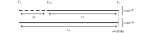
\includegraphics{figures/pep1_analys.pdf}
    \caption{Vehcile trajectories after the maneuver.}
    \label{fig:opt_res_num_pep1}
\end{figure}

$Y_{T0}$ and the speed at $Y_{T0}$, $v_{T0}$, assuming the same acceleration for both the vehicles from $Y_o$ to $Y_i$, is calculated by
\begin{align}
    Y_{T0} &= \frac{\mu g\left(\delta t\right)^2}{2} +  V_{y0(T)}\delta t + Y_o, & v_{T0} &= \mu g\delta t +  V_{y0(T)}.
\end{align}

For the intersection of the two cases to be even possible, 
\begin{align}
    v_{T0} &\leq V_{yo(V)}, & \mu g\delta t +  V_{y0(T)} &\leq V_{yo(V)},
\end{align}
where $V_{yo(V)}$ is the velocity at the end of the maneuver for case-V. 

For the intersection to be feasible, 
\begin{align}
    \mu &\leq \frac{V_{yo(V)} - V_{y0(T)}}{g\delta t}.\label{eq:mdl1}
\end{align}
Substituting the values of $g$, $\delta t$, $V_{yo(V)}$, and $V_{y0(T)}$ in \eqref{eq:mdl1}, $\mu \leq 0.158$. So icy conditions after the maneuver? Perhaps not. 

A deeper look into Figure~\ref{fig:pep1_part1}, shows that in case-V, there is little to no braking on the rear wheel of the rear wheel of the vehicle. This is perhaps the key to the pendulum turn being the time-optimal solution. 

\section{ST model with load transfer and maneuver change}

Unfortunately, implementing and recreating the results for the hairpin turn was very challenging and often lead to errors during optimization such as a reduction in alpha errors and so on.,... 
Therefore, a 90$^\circ$ tight right-hand turn was implemented and the constraint for the path in the OCP becomes
\begin{align}
    \left(\frac{X_P}{R_i}\right)^n + \left(\frac{Y_P}{R_i}\right)^n &\geq 1, &
    \left(\frac{X_P}{R_o}\right)^n + \left(\frac{Y_P}{R_o}\right)^n &\leq 1.
\end{align}
With this addition, the ipopt algorithm can find a solution for the OCP, without throwing any of the NaN found in the NLP error and so on. 

The normal forces acting on the wheels considering a load balancing between the front and the rear wheels for a given height of the vehicle's center of gravity ($h$) is 
\begin{align}
    F_{z(f)} &= \frac{mgl_r - hF_{X}}{l_r + l_f}, & F_{z(r)} &= \frac{mgl_f + hF_{X}}{l_r + l_f}.
\end{align}

\subsection{Load transfer vs static loads}
Figures~\ref{fig:pep2_comp_posplot} and \ref{fig:pep2_comp_detailplot} show the comparison between the ST-model with and without load transfer. From the figures it is clear that the LT model takes a longer time to complete the maneuver this is because of the effect of the load transfer, i.e., during acceleration, the maximum force on the front wheel is limited. 

\begin{figure}[h!]
    \centering
    \includegraphics{figures/pep2_comp_posplot.pdf}
    \caption{Time-optimal right-hand turn maneuver for ST model with and without load transfer. The rectangles indicate the position and direction of the vehicle each second.}
    \label{fig:pep2_comp_posplot}
\end{figure}

\begin{figure}[h!]
    \centering
    \includegraphics{figures/pep2_comp_detailplot.pdf}
    \caption{Variables of the vehicle model during the time-optimal right-hand turn maneuver with and without load transfer.}
    \label{fig:pep2_comp_detailplot}
\end{figure}

\subsection{Vopt vs. Topt}
As presented in the previous section, the output velocity optimized solution results in the pendulum turn Figures-\ref{fig:pep2_TVcomp_posplot} and \ref{fig:pep2_TVcomp_detailedplot} show the time optimal (topt) and velocity optimized (vopt) solutions for the right-hand turn maneuver for the ST-model with LT. 

\begin{figure}[h!]
    \centering
    \includegraphics{figures/pep2_TVcomp_posplot.pdf}
    \caption{Trajectory in the XY-plane for time and velocity optimized right-hand turn maneuver. The rectangles indicate the position and direction of the vehicle each second.}
    \label{fig:pep2_TVcomp_posplot}
\end{figure}

\begin{figure}[h!]
    \centering
    \includegraphics{figures/pep2_TVcomp_detailplot.pdf}
    \caption{Variables of the vehicle model during the time and velocity optimal right-hand turn maneuver.}
    \label{fig:pep2_TVcomp_detailedplot}
\end{figure}

The results of the final time and speed for the time and velocity optimal problem (Min $t$, and Max $v_f$) at the end of the maneuver are summarized in Table~\ref{tab:opt_res_num_pep2_TV}. 
From the table, it is clear that at $Y_o = 0$, Case-V (pendulum turn case) is about 1.5\,m/s faster but takes about 1\,s more to complete the maneuver. 
\begin{table}[h!]
    \centering
    \begin{tabular}{c|c|c|c}
        & & $t_f$ & $v_f$\\
        \hline
        \textbf{topt} & Min $t_f$ & 6.64\,s & 29.1 m/s (104.77\,km/h)\\
        \textbf{vopt} & Max $v_f$ & 8.15\,s & 29.66 m/s (106.78\,km/h)\\
    \end{tabular}
    \caption{Time and speed for the ST-model with LT for the two optimization cases topt and vopt the end of the maneuver, $Y_o = 0$.}
    \label{tab:opt_res_num_pep2_TV}
\end{table}

\clearpage
\subsection{Effect of road friction}
The road friction is changed to wet asphalt and snow conditions, the results are shown in Figures~\ref{fig:pep2_FricComp_posplot} and~\ref{fig:pep2_FricComp_posplot} From the figures, it is clear that the time and velocity optimized trajectories and velocity profiles are closer than for the case with dry and wet asphalt. 

\begin{figure}[h!]
    \centering
    \includegraphics{figures/pep2_FricComp_posplot.pdf}
    \caption{Trajectory in the XY-plane for time and velocity optimized right-hand turn maneuver for wet ahsplat and snow conditions. The rectangles indicate the position and direction of the vehicle each second.}
    \label{fig:pep2_FricComp_posplot}
\end{figure}

\begin{figure}[h!]
    \centering
    \includegraphics{figures/pep2_FricComp_detailplot.pdf}
    \caption{Variables of the vehicle model during the time and velocity optimal right-hand turn maneuver for wet asphalt and snow conditions.}
    \label{fig:pep2_FricComp_detailplot}
\end{figure}

\clearpage
The results of the final time and speed for the time and velocity optimal problem (Min $t$, and Max $v_f$) at the end of the maneuver for different road conditions are summarized in Table~\ref{tab:opt_res_num_pep2_fric}. 

\begin{table}[h!]
    \centering
    \begin{tabular}{c|c|c|c|c|c|c|c}
        & & \multicolumn{2}{c|}{Dry Asphalt} & \multicolumn{2}{c|}{Wet Asphalt} & \multicolumn{2}{c}{Snow}\\
        & & $t_f$ & $v_f$ & $t_f$ & $v_f$ & $t_f$ & $v_f$\\
        \hline
        \textbf{topt} & Min $t_f$ & 6.64\,s & 29.1 m/s & 6.86\,s & 27.68\,m/s & 10.9\,s & 17.64\,m/s\\
        & & & 104.77\,km/h & & 99.65\,km/h & & 63.49\,km/h\\
        \textbf{vopt} & Max $v_f$ & 8.15\,s & 29.66 m/s & 7.94\,s & 28.23\,m/s & 11.77\,s & 18.18\,m/s\\
        & & & 106.78\,km/h & & 101.69\,km/h & & 65.43\,km/h\\
    \end{tabular}
    \caption{Time and speed for the ST-model with LT for time and velocity optimized scenarios at the end of the maneuver, $Y_o = 0$, with different road frictions.}
    \label{tab:opt_res_num_pep2_fric}
\end{table}

From Figure~\ref{fig:pep2_FricComp_detailplot} it is clear that at no point in time is the velocity of the vehicle for vopt greater than topt but they do get close during snow conditions. This implies that the pendulum turn is not 'viable', even if there is a long straight after the maneuver. However, with a 9-DoF model with load transfer, one can perhaps observe the difference in acceleration of the pendulum turn (vopt) when compared to the time-optimal solution. 

\section*{Code}

The source codes for this problem can be found at \newline \href{https://github.com/arvba41/optimal_vehicle_maneuvers/blob/main/uppgift/pep1}{https://github.com/arvba41/optimal\_vehicle\_maneuvers}.

% \subsection{Effect of change in inertia}
% The mass and the inertia of the vehicle are increased by 12\,\%, and the results are shown in Figures~\ref{fig:pep2_FricComp_posplot} and~\ref{fig:pep2_FricComp_posplot} From the figures, it is clear that the time and velocity optimized trajectories and velocity profiles are closer than for the case with dry and wet asphalt. 
